\documentclass[12pt]{article}
\usepackage{amsmath}
\usepackage{listings}
\usepackage{color}
\usepackage{graphicx}
\title{Project 1}

\author{Dan Kolbman}
\date{September 22, 2014}

\definecolor{mygreen}{rgb}{0,0.6,0}
\definecolor{mygray}{rgb}{0.95,0.95,0.95}
\definecolor{mymauve}{rgb}{0.58,0,0.82}
%\definecolor{mygray}{RGB}{22, 22, 22}}

\lstset{ %
  language=Python,
  backgroundcolor=\color{mygray},   % choose the background color
  basicstyle=\footnotesize,        % size of fonts used for the code
  breaklines=true,                 % automatic line breaking only at whitespace
  captionpos=b,                    % sets the caption-position to bottom
  commentstyle=\color{mygreen},    % comment style
  %escapeinside={\%*}{*)},          % if you want to add LaTeX within your code
  keywordstyle=\color{blue},       % keyword style
  stringstyle=\color{mymauve},     % string literal style
  frame=L,
  xleftmargin=\parindent,
  showstringspaces=false
}
\begin{document}
  
  \maketitle

  \begin{equation}
    \label{eq:func}
    f(x) = x\left(1+\sum_{j=1}^{M}\frac{k_j\eta_j}{1+k_jx}\right)-\xi
  \end{equation}

  Define some test cases to user later: \\
  Case 1: \\
  $M=1$, $k=1$, $\eta=10$, $\xi=1$\\
  $x_r=0.099020$\\

  Case 2: \\
  $M=2$, $k_1=5$, $k_2=3$, $\eta_1=4$, $\eta_2=2$, $\xi=5$\\
  $x_r=0.63905$\\

  Case 3: \\
  $M=3$, $k_1=1$, $k_2=2$, $k_3=6$, $\eta_1=2$, $\eta_2=3$, $\eta_3=1$, $\xi=9$\\
  $x_r=3.8064$\\

  \subsection*{Plot for $M = 1, k=1, \eta=1, \xi = 3$}

  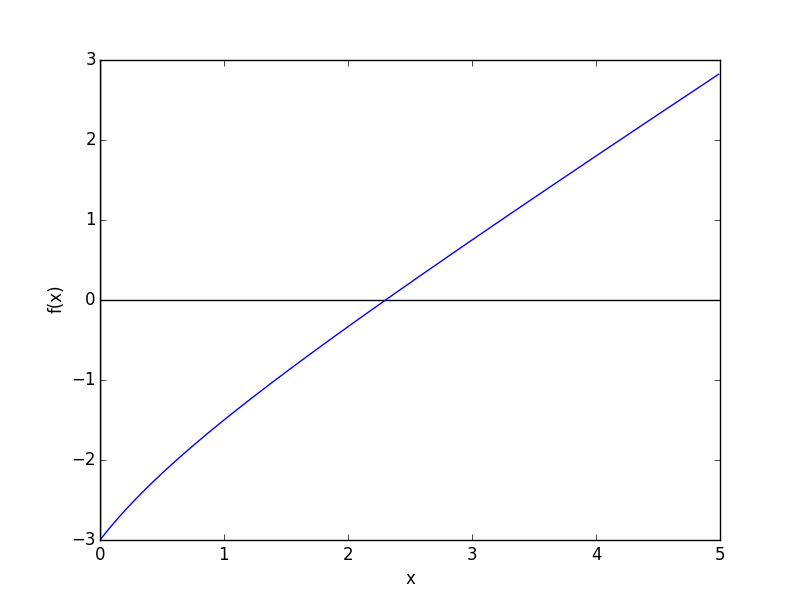
\includegraphics[scale=0.65]{plot1.png}

  \clearpage

  \subsection*{Show that Eq. \ref{eq:func} is Negative for $x=0$}

  If $x=0$:
  
  \begin{align}
    f(0) &= x\left(1+\sum_{j=1}^{M}\frac{k_j\eta_j}{1+k_j0}\right)-\xi\nonumber\\
    f(0) &=  - \xi    \nonumber
  \end{align}

  Where $\xi > 0$, as the concentration can not be negative. Thus,

  \begin{align}
    \label{eq:a}
    f(0) < 0
  \end{align}

  \subsection*{Eq. \ref{eq:func} is Strictly Increasing for $x>0$ }

  We can show that $f(x)$ is constantly increasing by observing that the
  derivative is positive for $x>0$:
  \begin{align}
    \frac{df(x)}{dx} &= 1+\frac{d}{dx}\left(\sum_{j=1}^{M}\frac{xk_j\eta_j}{1+k_jx}\right) &\nonumber\\
    \frac{df(x)}{dx} &= 1 + \sum_{j=1}^{M}\frac{k_j\eta_j}{(1+k_jx)^2} &\nonumber\\
    \label{eq:b}
    \frac{df(x)}{dx} &> 0 & \forall (x > 0)\in \Re &
  \end{align}

  \subsection*{Eq. \ref{eq:func} is Positive for for large $x$}
  
  Given that the derivative is alway positive, there must be some point at which,

  \begin{align}
    \label{eq:c}
    f(x) > 0, x \to \infty
  \end{align}

  \subsection*{Eq. \ref{eq:func} Always has one Positive Solution}
  
  Given conditions \ref{eq:a}, \ref{eq:b}, and \ref{eq:c}, there must exist one
  value of $x>0$ for which $f(x) = 0$.

  

  \subsection*{Bisection}

  \subsection*{Fixed Point Iteration}

  \begin{equation}
    \label{eq:fpi1}
    x = \xi - x \sum_{j=1}^M\frac{k_j\eta_j}{1+k_jx}=g(x)
  \end{equation}

  The root of

  $$x(1+\frac{1}{1+x}) - 3= 0 $$

  Using FPI and Eq. \ref{eq:fpi1} to obtain a $g(x)$:

  $$g(x) = 3 - \frac{x}{1+x} $$

  which correctly converges to 2.30277.

  However, using the form of Eq. \ref{eq:fpi1} to find the root of

  $$x(1+\frac{5}{1+x}) - 3 = 0 $$

  with a $g(x)$:
  
  $$ g(x) = 3 - \frac{5x}{1+x} $$

  By inspecting $|g'(x)|$ at the desired root we see, for the second case, that:
  $$g'(0.79129) = |\frac{5}{(x+1)^2}| = 1.558 $$
  Which indicates that it diverges since it is greater than one.
  Compare with the first case where we see that:
  $$g'(2.30277) = |\frac{1}{(x+1)^2}| = 0.0918 $$
  Thus implying convergence (which it does) as it is less than one.\\
  \\
  Now using a definition of $g_\alpha(x)$:
  
  \begin{equation}
    \label{eq:ga}
    g_\alpha(x) = \frac{1}{1+\alpha}\left[\xi+x\left(\alpha-\sum_{j=1}^{M}\frac{k_j\eta_j}{1+k_jx}\right)\right]=x
  \end{equation}

  We can find an $\alpha$ such that $|g_\alpha'(r)|<1$ so that we will have
  convergence:
  
  $$g_\alpha (x) = \frac{1}{1+\alpha}\left[3+x(\alpha-\frac{5}{1+x}\right] $$

  $$g_\alpha'(x) = \frac{1}{1+\alpha}\frac{\alpha(x+1)^2-5}{(x+1)^2} $$

  $$g_\alpha'(2.30277) = \frac{\alpha - 0.45836}{1+\alpha} $$

  Thus, to gurantee convergence, we find that $\alpha > 0.27$ (by finding the
  root of $g_\alpha'(2.30277)-1=0$).
  With a value of $\alpha=1$, the root for the second case correctly converges
  to $x=0.79128$.

  \subsection*{Newton's Method}
  \subsubsection*{Consider Eq. \ref{eq:func} for $M=1$, $k=1$, $\eta=1$, and $\xi=3$:}

  For an initial guess $x_0=1.6$, Newton's Method will converge on a root,
  howerver, it is the root at $x=-10.099$ rather than the root closer to the
  initial guess at $x=0.099$.

  When choosing $x_0=1.4999$, the next guess still overestimates the root, but
  not badly enough to jump over the asymptote and converge on a different root.

  When starting from $x_0=1.5$. the next guess will land very close to the
  asymptote and many small steps are spent moving down the steep slope until
  it eventually reaches the root.
  
  The guess following $x_0=1$ lies closest to the root due to the down
  concavity as the function approaches the root. This results in the following
  guesses being close to the root where there is no extreme slopes and will
  quickly converge.

  \subsubsection*{Consider Eq. \ref{eq:func} for $M=3$, $\xi=9$, $k_1=1, k_2=2, k_3=6$
  $\eta_1=2, \eta_2=3, \eta_3=1$:}

  The function is nearly linear for values of $x > 0$ so Newton's Method
  converges very quickly. For initial values of $x_0 < 0$ but greater than 
  the asyptote, more iterations will be needed, but the function will still
  converge on $x=3.086$.

  \subsection*{Comparison Between Methods}

  Bisection, FPI, and Newton's Method were applied to each of the three test
  cases listed at the begining. Bisection and FPI methods both converged linearly
  on the roots. Bisection took about 40 steps to converge on
  the roots, while FPI took between 15-25. Newton's method converged quadratically
  never taking more than 5 steps to converge within tolerance.

  Clearly the quadratically convergent Newton's method is the best solution
  to finding roots of this type.

  
  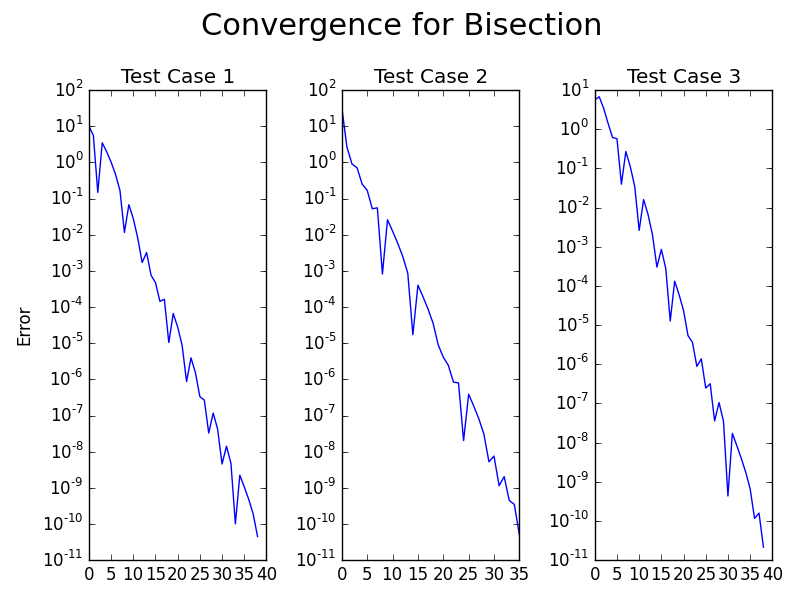
\includegraphics[scale=0.65]{bisect_tests.png}\\
  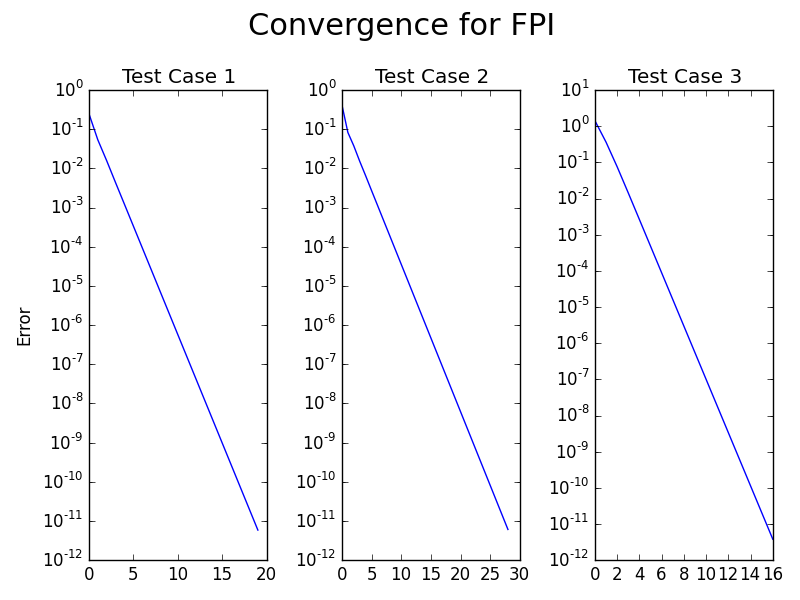
\includegraphics[scale=0.65]{fpi_tests.png}\\
  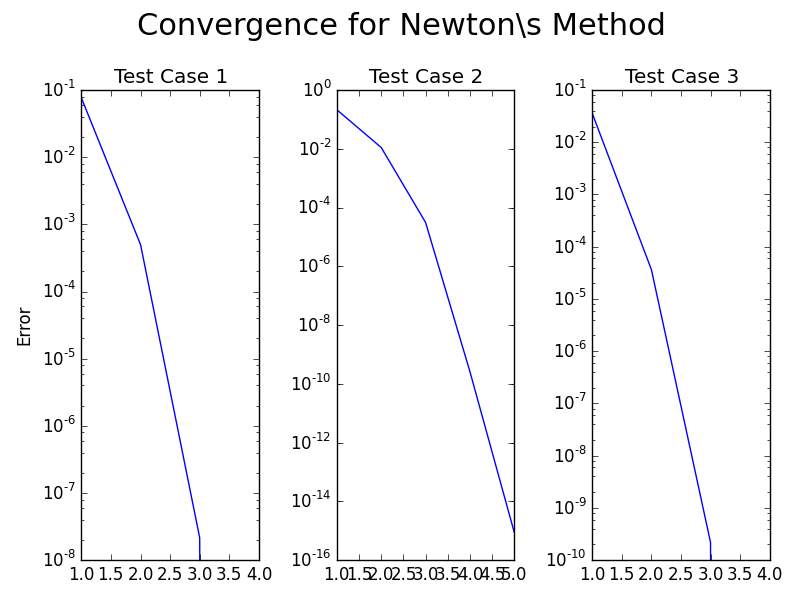
\includegraphics[scale=0.65]{newton_tests.png}
  
  
\end{document}
